\url{http://cms.avg-hrd.appspot.com/securitycenter/securitypost_20110927.html}

\section{Overview}

\textbf{Name:} Gone in 60 Seconds \\
\textbf{Malware type:} Spyware \\
\textbf{Geo:} All around \\
\textbf{Score:} 3 \\
\textbf{Date Discovered:} 24.09.2011 \\
\textbf{Date Added:} 24.09.2011 \\

An Android application that can used as a spyware was found on Android Market

The application is Android cloud spyware that can be used by an attacker or not authorized user to take out personal info from the device such as contacts, messages, recent calls and history.

\section{Geeks Info}

\textbf{Method of Infection:} Installing an APK file \\
\textbf{Encrypted:} No \\
\textbf{Distribution Potential:} Low \\
\textbf{In the wild:} Yes \\
\textbf{Overall Risk Rating:} Low \\
\textbf{Damage Potential:} Low \\
\textbf{Reverse info:} Available \\
\textbf{Symptoms:} Taking personal information from target phone \\

\parbox{\textwidth}{
The developer of the app is 'CreativeDogs': \\
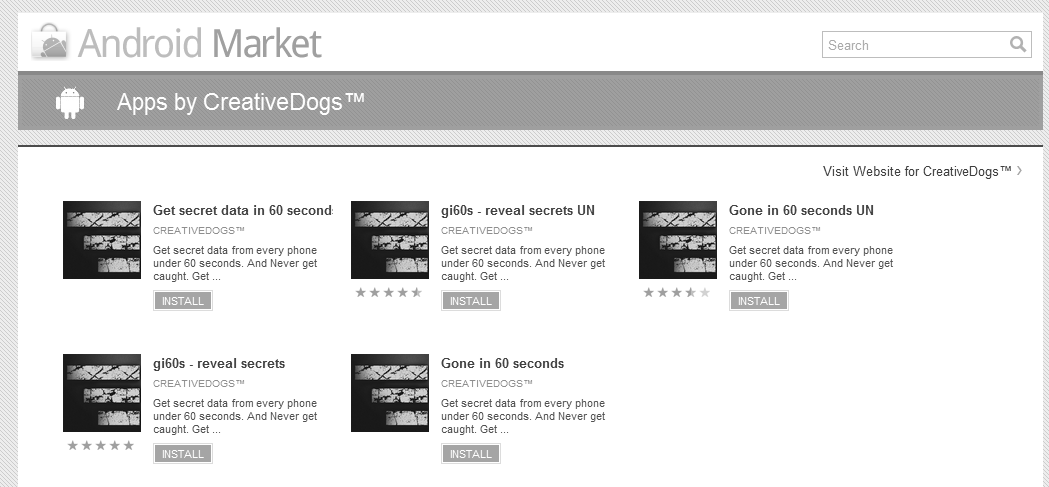
\includegraphics[width=0.95\textwidth]{figs/gone60_1.png}
}

\parbox{\textwidth}{
Details taken from the market: \\
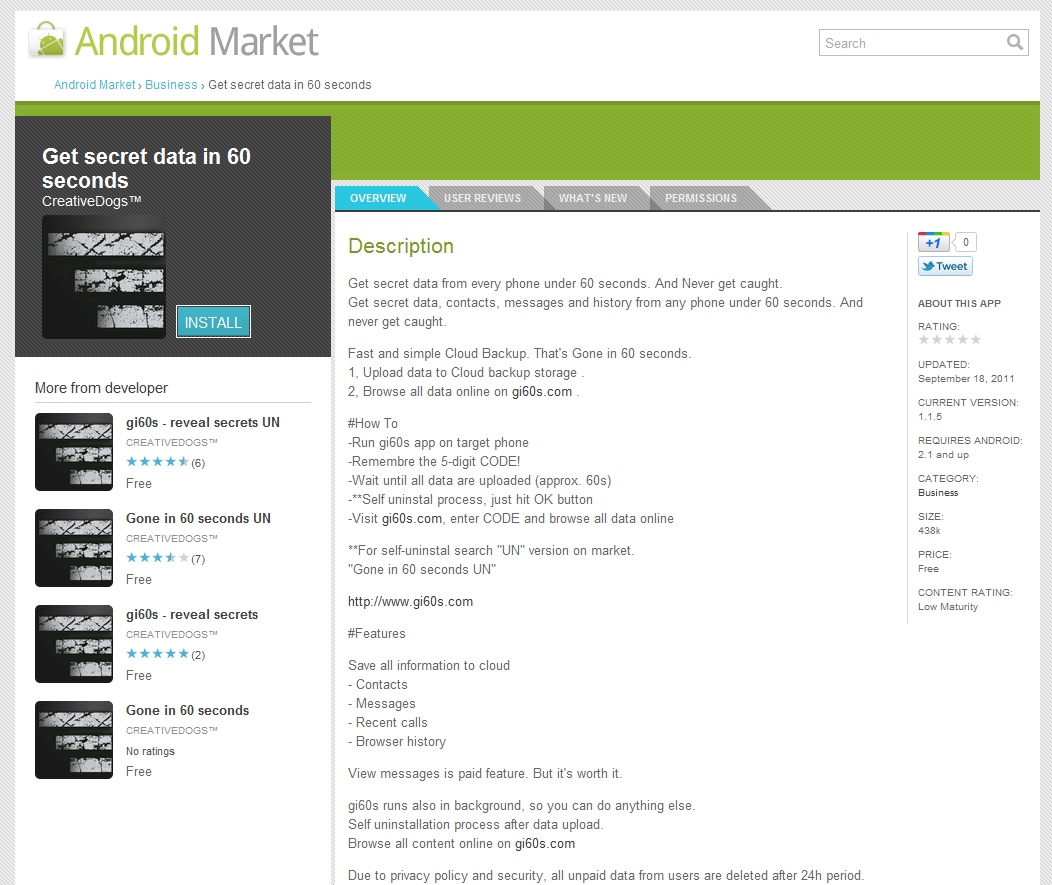
\includegraphics[width=0.95\textwidth]{figs/gone60_2.png}
}

\subsubsection{Package name}
\parbox{\textwidth}{
The package name of the application is 'com.gone603': \\
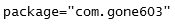
\includegraphics[width=0.3\textwidth]{figs/gone60_3.png} \\
\emph{Notice:} there are few variants of this app.
}

\subsubsection{Permissions}
\parbox{\textwidth}{
The spyware requests the permissions needed to what it intended to do: \\
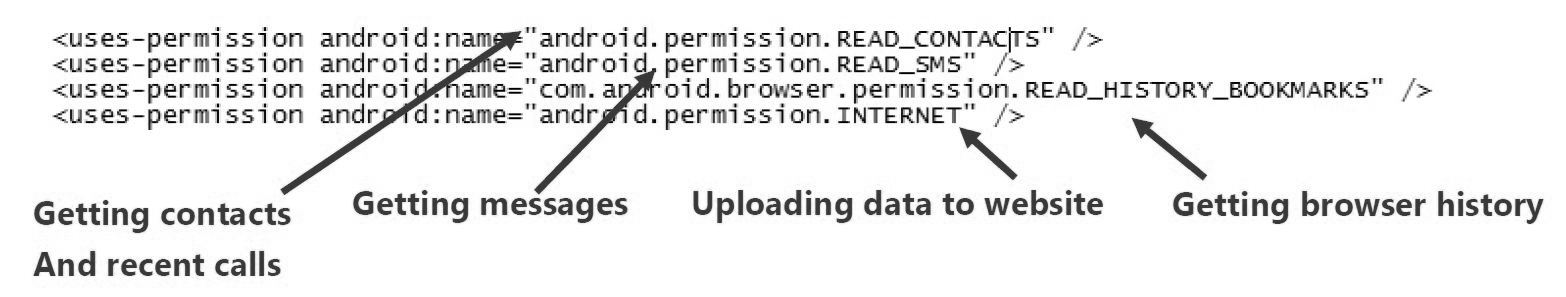
\includegraphics[width=\textwidth]{figs/gone60_4.JPG}
}

\subsubsection{Installing}
To activate the spyware the attacker needs to download and install it on the target phone.

\subsubsection{5 digit code}
\parbox{\textwidth}{
To activate the application the user needs to run it and remember the 5-digit code that will be later be used to browse the personal info taken in the spyware author. Below you can see how the application looks when running - the red area covers the code generated by the application: \\
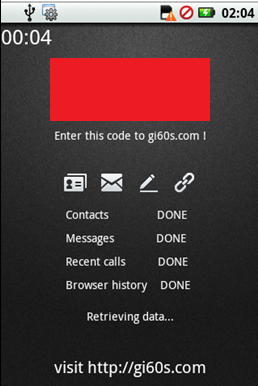
\includegraphics[width=0.5\textwidth]{figs/gone60_5.png}
}

\subsubsection{Running in the background}
The application runs in the background.

\subsubsection{Taking personal information from the target phone}
\parbox{\textwidth}{
The application gets its name from the time it takes for getting the data ad upload it to the spyware author's website. The flow and timing described below: \\
\texttt{Cloning contacts.. (10s)} \\
\texttt{Cloning messages.. (20s)} \\
\texttt{Cloning recent calls.. (10s)} \\
\texttt{Cloning browser history.. (15s)} \\
\texttt{Uploading data to gi60s.com.. (5s)} \\
}

\parbox{\textwidth}{
Here we can see the code part that is responsible for the flow: \\
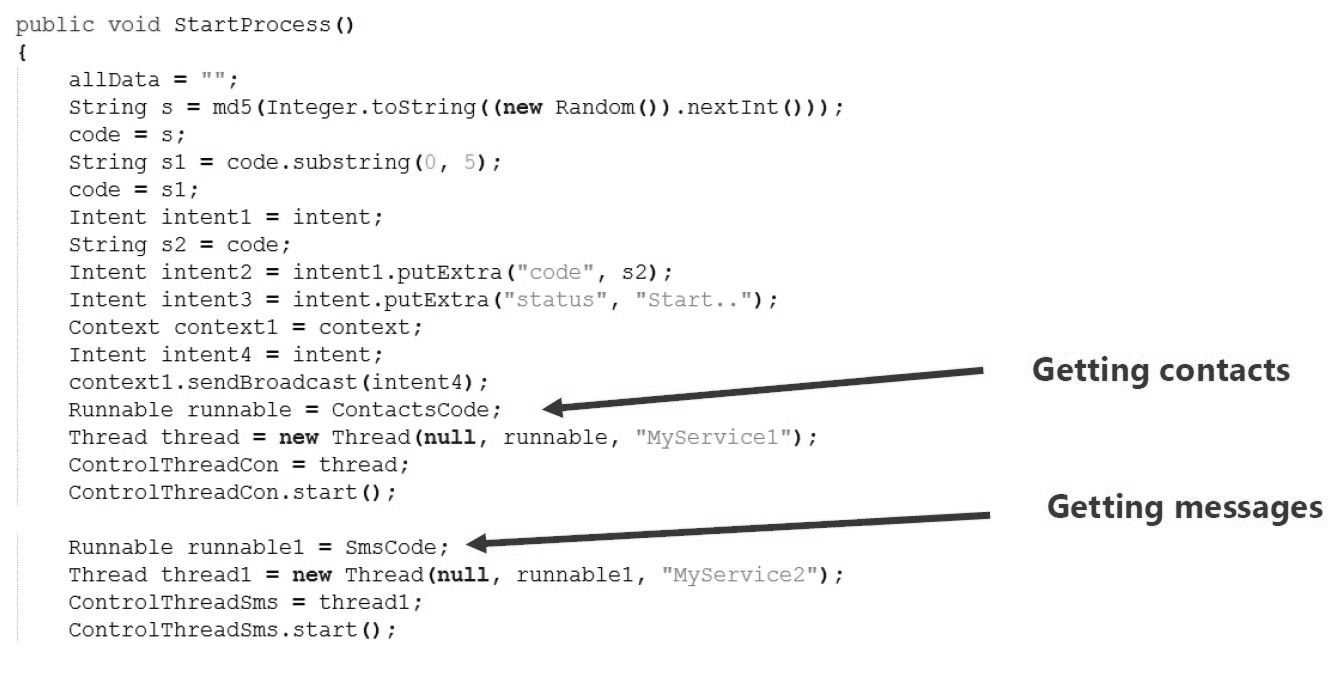
\includegraphics[width=\textwidth]{figs/gone60_6.JPG} \\
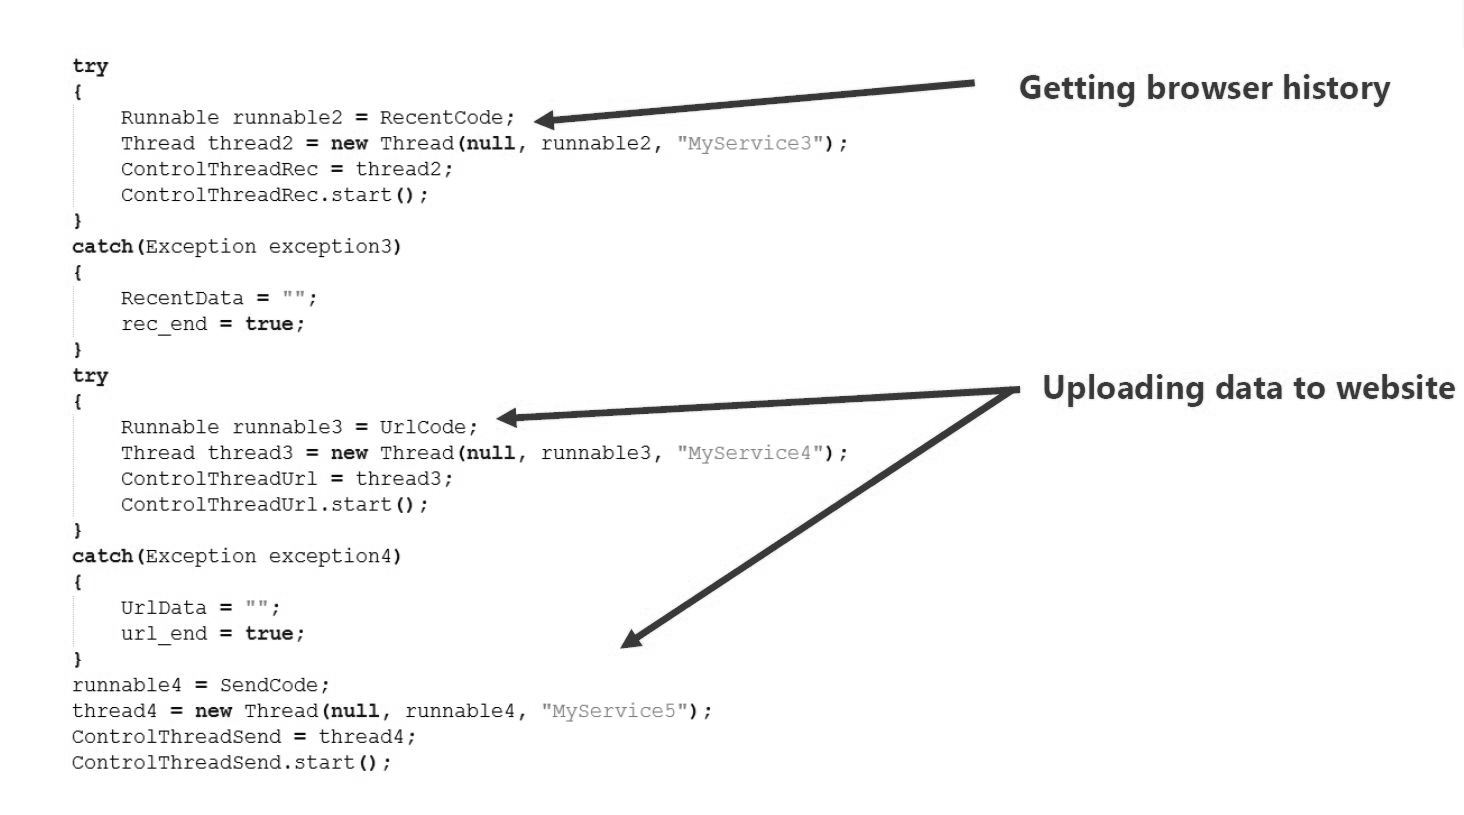
\includegraphics[width=\textwidth]{figs/gone60_6_2.JPG}
}

\parbox{\textwidth}{
Here we can see the code that takes the contacts (name + number) from the target phone: \\
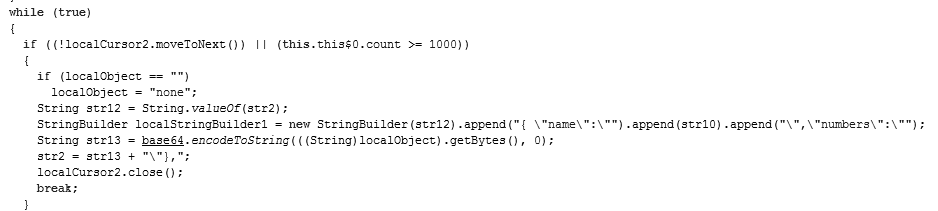
\includegraphics[width=\textwidth]{figs/gone60_7.png}
}

\parbox{\textwidth}{
Here we can see the code that takes the messages: \\
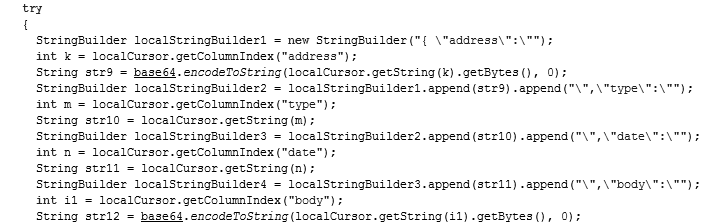
\includegraphics[width=\textwidth]{figs/gone60_8.png}
}

\parbox{\textwidth}{
Here we can see the code that takes the recent calls: \\
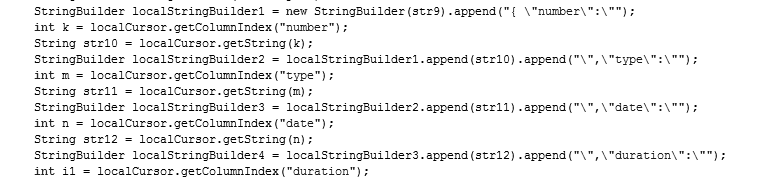
\includegraphics[width=\textwidth]{figs/gone60_9.png}
}

\parbox{\textwidth}{
Here we can see the code that takes the recent history: \\
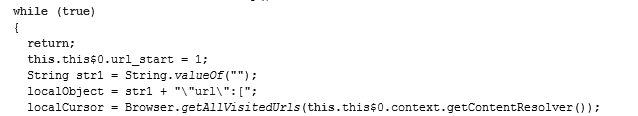
\includegraphics[width=\textwidth]{figs/gone60_10.png}
}

\subsubsection{Self-uninstallation}
\parbox{\textwidth}{
The developer declares that "The app automatically starts process of self-uninstallation". In reality, after running it the application still can be found on the device: \\
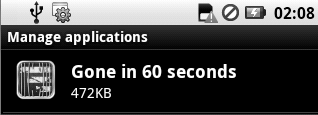
\includegraphics[width=0.5\textwidth]{figs/gone60_11.png}
}

\subsubsection{Getting the information taken from the target phone}
When you want to see the info taken from the device you need to browse to the application author website (giXXs.com), enter code and browse all contacts. To browse also messages, recent calls and history you need to pay the author 5\$.

\parbox{\textwidth}{
Here we can see the hard coded url of the author's website: \\
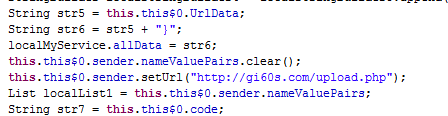
\includegraphics[width=\textwidth]{figs/gone60_12.png}
}

\parbox{\textwidth}{
When you browse to the website there's a menu offer options: \\
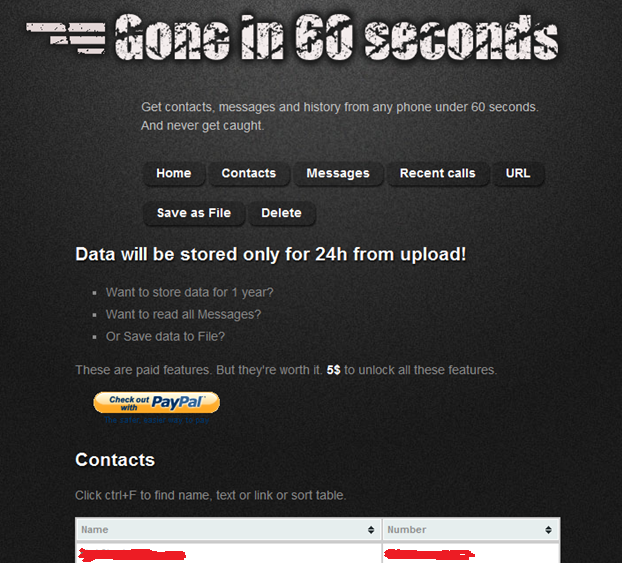
\includegraphics[width=0.75\textwidth]{figs/gone60_13.png}
}

\parbox{\textwidth}{
The authors of the application declare that the data will be stored only for 24h from upload. \\
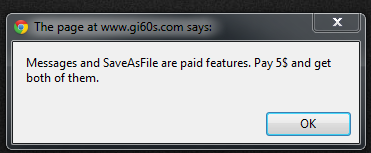
\includegraphics[width=0.5\textwidth]{figs/gone60_14.png}
}

\parbox{\textwidth}{
The following picture was taken from the author's website:\\
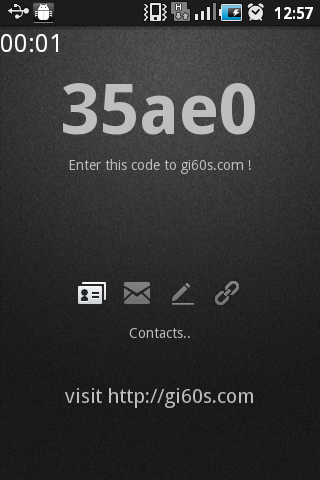
\includegraphics[width=0.5\textwidth]{figs/gone60_15.png}
}
